\part{Praktická část}

\chapter{Cíl projektu}

V praktické části mé práce jsem vytvořil vlastní hru pro VR. Stanovil jsem si následující kritéria:

\begin{itemize}
	\item \textbf{Nenáročnost}. Chtěl jsem, aby má hra nebyla obtížná na pochopení. Většina VR her vyžaduje zvýšenou fyzickou aktivitu nebo hlubší porozumění VR konceptů. Ideálně jsem chtěl vytvořit hru, kterou bych mohl komukoliv půjčit, aniž bych musel dlouze vysvětlovat její princip.
  \item \textbf{Grafická jednoduchost}. Nepovažuji se za umělce a umím vytvářet pouze základní modely a textury. Bylo pro mě tedy klíčové přijít s takovým konceptem, který by byl vzhledově nenáročný.
  \item \textbf{Interaktivita}. Od své hry jsem chtěl, aby doopravdy využívala funkce, které VR platformy poskytují. Tedy ovládání pohybem, jednoduchá fyzika atp.
\end{itemize}

Dospěl jsem k následujícímu návrhu: Hra sestává z kostky tvořené úrovněmi nakládanými na sebe. Každá úroveň představuje bludiště, skrze které musí nakláněním hráč navigovat kuličku. Při dosažení cíle je úroveň odebrána, kostka se zmenší a je odhalena další úroveň.

To splňuje moje kritéria - hra je jednoduchá, na vykreslení potřebuje jen geometrické tvary a vyžaduje pohyb rukama pro naklánění bludiště.

Již od samého začátku jsem svou hru chtěl napsat v herním enginu. Herních enginů zdarma, které zároveň podporují XR, není mnoho. Zvolil jsem si svobodný Godot Engine.

\chapter{Herní engine Godot}

Godot je bezplatný herní engine. Hlavní důvod, proč jsem si ho vybral namísto známějšího Unity, je jeho licence. Godot je šířen pod svobodnou licencí MIT, která vývojářům dovoluje kód používat komerčně i naopak, a to pod jedinou podmínkou: text licence je ve výsledné práci zachován. Unity Engine je naopak distribuován pod nesvobodnou licencí a za některé funkce musí vývojáři platit. Godot se v poslední době stává více a více populárním a obdržel investice od velkých společností. Mezi ně patří např. grant od Epic Games pro vývoj grafiky a grant od Mety pro vývoj XR funkcí. \cite{godot_epicgames} \cite{godot_meta}

\section{Struktura Godot projektu}

Pro úpravu Godot projektů používáme oficiální editor. Objekty v projektu jsou reprezentovány jako strom uzlů, podobně jako jsou webové stránky reprezentovány stromem značek. Uzly samy o sobě nemají velkou hodnotu, ale jejich kombinováním můžeme dosáhnout komplexnější logiky. Části stromů můžeme dále uložit jako \textit{scénu} (textový soubor .tscn), kterou můžeme poté instancovat.

\begin{figure}[H]
  \centering
  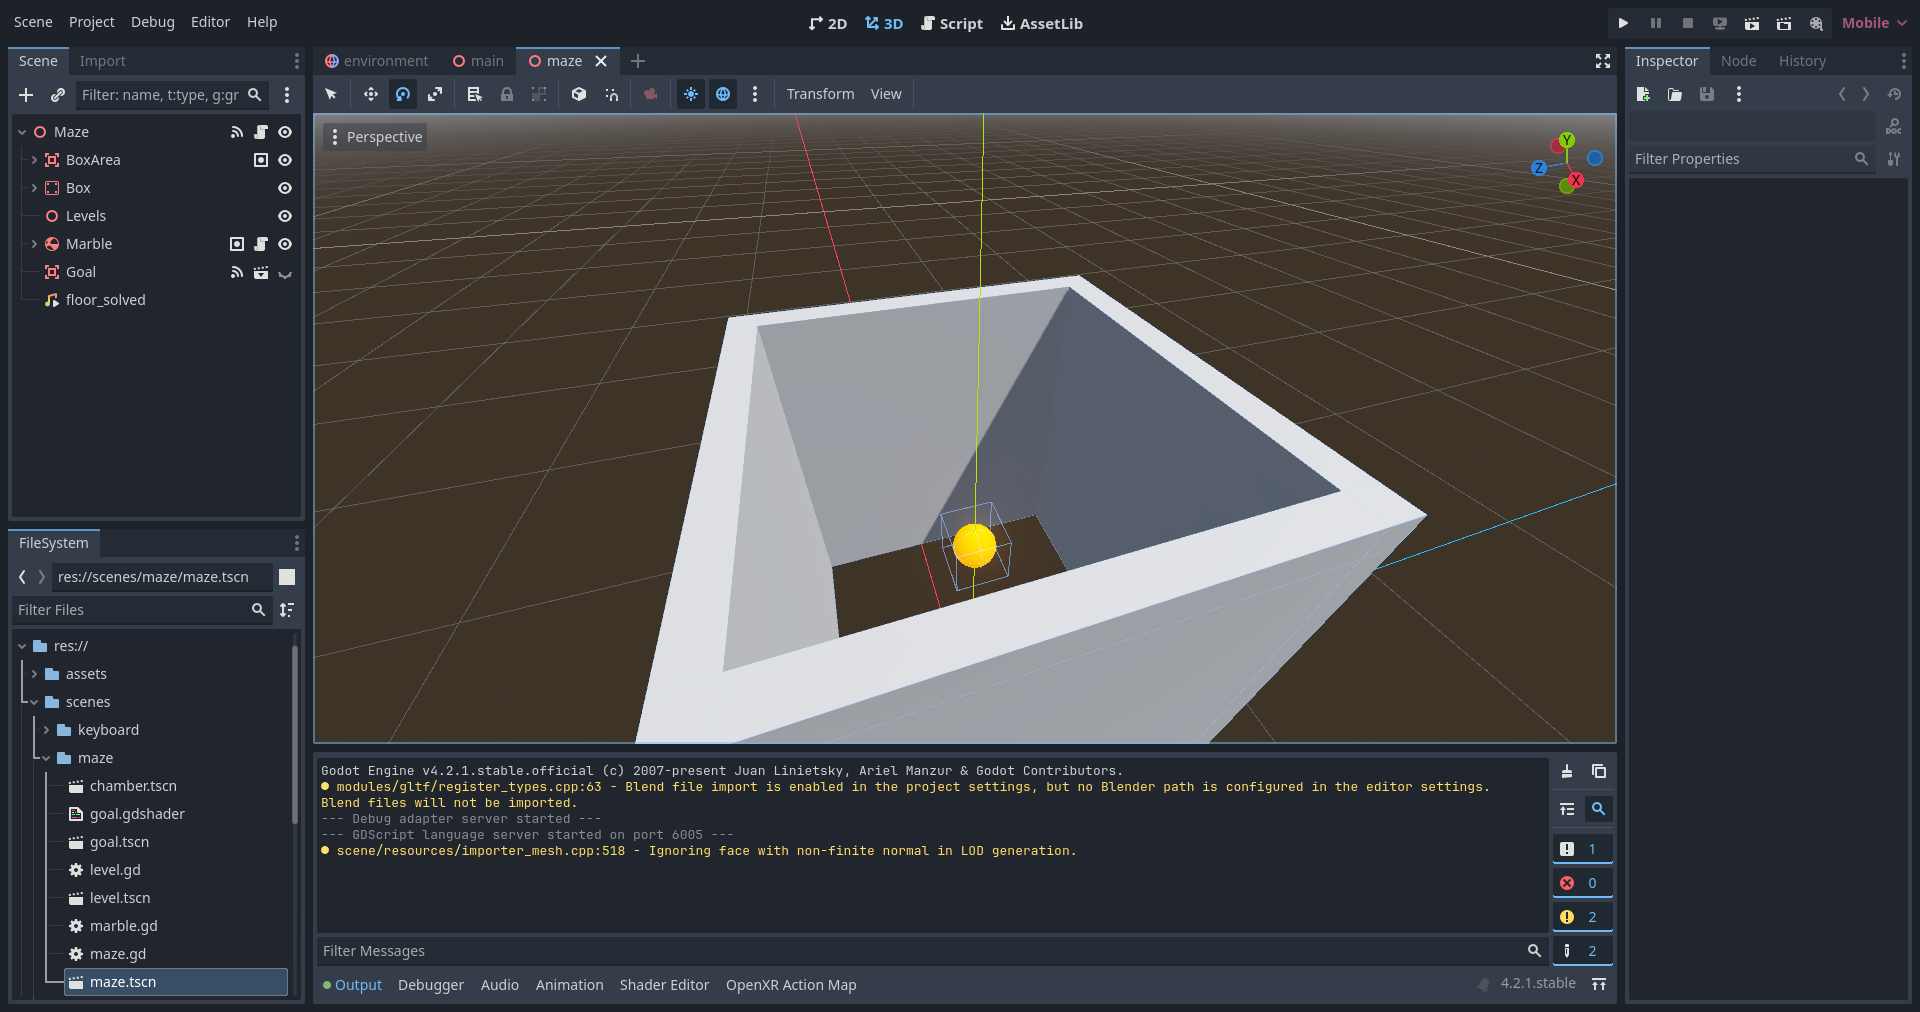
\includegraphics[height=180pt]{godot_editor.png}
  \caption{Editor Godot Engine a otevřená scéna Maze.tscn}
  \label{godot_editor_maze_tscn}
\end{figure}

\section{Jazyk \textit{GDScript}}

\chapter{Algoritmy}

\section{Generování bludiště}

\chapter{Interaktivita}

\section{Manipulace s bludištěm}

\section{Uživatelské rozhraní}
